\documentclass[tikz,border=10pt]{standalone}
\usepackage{tikz}
\usetikzlibrary{positioning,shapes.geometric,arrows.meta,calc}

\begin{document}
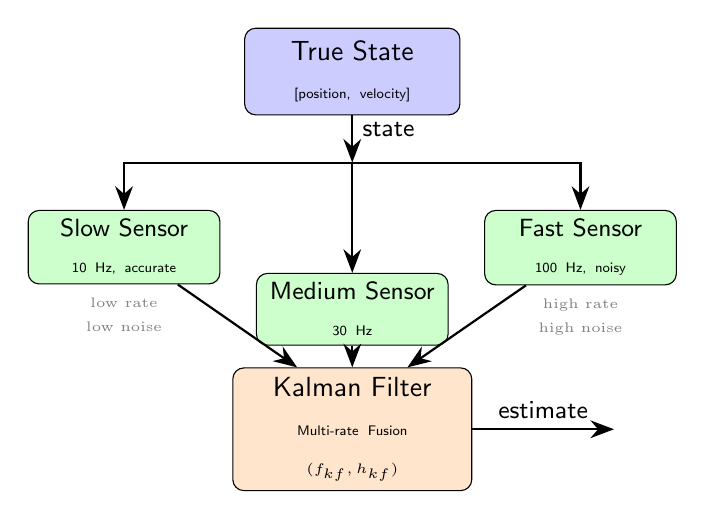
\begin{tikzpicture}[
    node distance=2.5cm,
    block/.style={rectangle, draw, fill=blue!20, text width=2.5cm, text centered, rounded corners, minimum height=1.1cm, font=\sffamily},
    sensor/.style={rectangle, draw, fill=green!20, text width=2.2cm, text centered, rounded corners, minimum height=0.9cm, font=\sffamily\small},
    kf/.style={rectangle, draw, fill=orange!20, text width=2.8cm, text centered, rounded corners, minimum height=1.3cm, font=\sffamily},
    arrow/.style={-{Stealth[length=3mm]}, thick},
    signal/.style={font=\small\sffamily}
]

% Plant
\node[block] (plant) {True State\\[2pt]{\tiny [position, velocity]}};

% Sensors at different rates
\node[sensor, below right=1.2cm and 0.3cm of plant] (fast) {Fast Sensor\\[2pt]{\tiny 100 Hz, noisy}};
\node[sensor, below=2.0cm of plant] (medium) {Medium Sensor\\[2pt]{\tiny 30 Hz}};
\node[sensor, below left=1.2cm and 0.3cm of plant] (slow) {Slow Sensor\\[2pt]{\tiny 10 Hz, accurate}};

% Kalman filter
\node[kf, below=3.2cm of plant] (kf) {Kalman Filter\\[2pt]{\tiny Multi-rate Fusion}\\[2pt]{\tiny $(f_{\text{kf}}, h_{\text{kf}})$}};

% Output
\coordinate[right=1.8cm of kf] (output);

% Branching point from plant
\coordinate[below=0.6cm of plant] (branch);

% Arrows from plant to sensors
\draw[arrow] (plant) -- node[right, signal, pos=0.3] {state} (branch);
\draw[arrow] (branch) -| (fast);
\draw[arrow] (branch) -- (medium);
\draw[arrow] (branch) -| (slow);

% Arrows from sensors to KF
\draw[arrow] (fast) -- ($(kf.north)+(0.7,0)$);
\draw[arrow] (medium) -- (kf.north);
\draw[arrow] (slow) -- ($(kf.north)+(-0.7,0)$);

% Arrow from KF to output
\draw[arrow] (kf) -- node[above, signal] {estimate} (output);

% Rate annotations
\node[below=0.05cm of fast, signal, font=\tiny, text=gray] {high rate};
\node[below=0.05cm of fast, signal, font=\tiny, text=gray, yshift=-0.3cm] {high noise};
\node[below=0.05cm of slow, signal, font=\tiny, text=gray] {low rate};
\node[below=0.05cm of slow, signal, font=\tiny, text=gray, yshift=-0.3cm] {low noise};

\end{tikzpicture}
\end{document}
